%%%%%%%%%%%%%%%%%%%%%%%%%%%%%%%%%%%%%%%%%
% Programming/Coding Assignment
% LaTeX Template
%
% This template has been downloaded from:
% http://www.latextemplates.com
%
% Original author:
% Ted Pavlic (http://www.tedpavlic.com)
%
% Note:
% The \lipsum[#] commands throughout this template generate dummy text
% to fill the template out. These commands should all be removed when 
% writing assignment content.
%
% This template uses a Perl script as an example snippet of code, most other
% languages are also usable. Configure them in the "CODE INCLUSION 
% CONFIGURATION" section.
%
%%%%%%%%%%%%%%%%%%%%%%%%%%%%%%%%%%%%%%%%%

%----------------------------------------------------------------------------------------
%	PACKAGES AND OTHER DOCUMENT CONFIGURATIONS
%----------------------------------------------------------------------------------------

\documentclass{article}

\usepackage{fancyhdr} % Required for custom headers
\usepackage{lastpage} % Required to determine the last page for the footer
\usepackage{extramarks} % Required for headers and footers
\usepackage[usenames,dvipsnames]{color} % Required for custom colors
\usepackage{graphicx} % Required to insert images
\usepackage{listings} % Required for insertion of code
\usepackage{courier} % Required for the courier font
\usepackage{lipsum} % Used for inserting dummy 'Lorem ipsum' text into the template
\usepackage{setspace}
\usepackage{color}
\usepackage{comment}
\usepackage{caption}

\usepackage{hyperref}
\usepackage{natbib}
\usepackage{underscore}
\usepackage{subfigure}
\usepackage{fixltx2e}

\hypersetup{
    colorlinks=true,
    linkcolor=blue,
    filecolor=magenta,      
    urlcolor=cyan,
    breaklinks=true
}

%\usepackage[]{algorithm2e}
\usepackage{pdfpages}




%For python inclusion (http://widerin.org/blog/syntax-highlighting-for-python-scripts-in-latex-documents)
\definecolor{Code}{rgb}{0,0,0}
\definecolor{Decorators}{rgb}{0.5,0.5,0.5}
\definecolor{Numbers}{rgb}{0.5,0,0}
\definecolor{MatchingBrackets}{rgb}{0.25,0.5,0.5}
\definecolor{Keywords}{rgb}{0,0,1}
\definecolor{self}{rgb}{0,0,0}
\definecolor{Strings}{rgb}{0,0.63,0}
\definecolor{Comments}{rgb}{0,0.63,1}
\definecolor{Backquotes}{rgb}{0,0,0}
\definecolor{Classname}{rgb}{0,0,0}
\definecolor{FunctionName}{rgb}{0,0,0}
\definecolor{Operators}{rgb}{0,0,0}
\definecolor{Background}{rgb}{0.98,0.98,0.98}

% Margins
\topmargin=-0.45in
\evensidemargin=0in
\oddsidemargin=0in
\textwidth=6.5in
\textheight=9.0in
\headsep=0.25in

\linespread{1.1} % Line spacing

% Set up the header and footer
\pagestyle{fancy}
\lhead{\hmwkAuthorName} % Top left header
%\chead{\hmwkClass\ (\hmwkClassInstructor\ \hmwkClassTime): \hmwkTitle} % Top center head
\chead{\hmwkClass\ (\hmwkClassInstructor): \hmwkTitle} % Top center head
\rhead{\firstxmark} % Top right header
\lfoot{\lastxmark} % Bottom left footer
\cfoot{} % Bottom center footer
\rfoot{Page\ \thepage\ of\ \protect\pageref{LastPage}} % Bottom right footer
\renewcommand\headrulewidth{0.4pt} % Size of the header rule
\renewcommand\footrulewidth{0.4pt} % Size of the footer rule

\setlength\parindent{0pt} % Removes all indentation from paragraphs

%----------------------------------------------------------------------------------------
%	CODE INCLUSION CONFIGURATION
%----------------------------------------------------------------------------------------

\definecolor{MyDarkGreen}{rgb}{0.0,0.4,0.0} % This is the color used for comments
\lstloadlanguages{Perl} % Load Perl syntax for listings, for a list of other languages supported see: ftp://ftp.tex.ac.uk/tex-archive/macros/latex/contrib/listings/listings.pdf
\lstset{language=Perl, % Use Perl in this example
        frame=single, % Single frame around code
        basicstyle=\small\ttfamily, % Use small true type font
        keywordstyle=[1]\color{Blue}\bf, % Perl functions bold and blue
        keywordstyle=[2]\color{Purple}, % Perl function arguments purple
        keywordstyle=[3]\color{Blue}\underbar, % Custom functions underlined and blue
        identifierstyle=, % Nothing special about identifiers                                         
        commentstyle=\usefont{T1}{pcr}{m}{sl}\color{MyDarkGreen}\small, % Comments small dark green courier font
        stringstyle=\color{Purple}, % Strings are purple
        showstringspaces=false, % Don't put marks in string spaces
        tabsize=5, % 5 spaces per tab
        %
        % Put standard Perl functions not included in the default language here
        morekeywords={rand},
        %
        % Put Perl function parameters here
        morekeywords=[2]{on, off, interp},
        %
        % Put user defined functions here
        morekeywords=[3]{test},
       	%
        morecomment=[l][\color{Blue}]{...}, % Line continuation (...) like blue comment
        numbers=left, % Line numbers on left
        firstnumber=1, % Line numbers start with line 1
        numberstyle=\tiny\color{Blue}, % Line numbers are blue and small
        stepnumber=5 % Line numbers go in steps of 5
}

% Creates a new command to include a perl script, the first parameter is the filename of the script (without .pl), the second parameter is the caption
\newcommand{\perlscript}[2]{
\begin{itemize}
\item[]\lstinputlisting[caption=#2,label=#1]{#1.pl}
\end{itemize}
}


%----------------------------------------------------------------------------------------
%	DOCUMENT STRUCTURE COMMANDS
%	Skip this unless you know what you're doing
%----------------------------------------------------------------------------------------

% Header and footer for when a page split occurs within a problem environment
\newcommand{\enterProblemHeader}[1]{
\nobreak\extramarks{#1}{#1 continued on next page\ldots}\nobreak
\nobreak\extramarks{#1 (continued)}{#1 continued on next page\ldots}\nobreak
}

% Header and footer for when a page split occurs between problem environments
\newcommand{\exitProblemHeader}[1]{
\nobreak\extramarks{#1 (continued)}{#1 continued on next page\ldots}\nobreak
\nobreak\extramarks{#1}{}\nobreak
}

\setcounter{secnumdepth}{0} % Removes default section numbers
\newcounter{homeworkProblemCounter} % Creates a counter to keep track of the number of problems

\newcommand{\homeworkProblemName}{}
\newenvironment{homeworkProblem}[1][Problem \arabic{homeworkProblemCounter}]{ % Makes a new environment called homeworkProblem which takes 1 argument (custom name) but the default is "Problem #"
\stepcounter{homeworkProblemCounter} % Increase counter for number of problems
\renewcommand{\homeworkProblemName}{#1} % Assign \homeworkProblemName the name of the problem
\section{\homeworkProblemName} % Make a section in the document with the custom problem count
\enterProblemHeader{\homeworkProblemName} % Header and footer within the environment
}{
\exitProblemHeader{\homeworkProblemName} % Header and footer after the environment
}

\newcommand{\problemAnswer}[1]{ % Defines the problem answer command with the content as the only argument
\noindent\framebox[\columnwidth][c]{\begin{minipage}{0.98\columnwidth}#1\end{minipage}} % Makes the box around the problem answer and puts the content inside
}

\newcommand{\homeworkSectionName}{}
\newenvironment{homeworkSection}[1]{ % New environment for sections within homework problems, takes 1 argument - the name of the section
\renewcommand{\homeworkSectionName}{#1} % Assign \homeworkSectionName to the name of the section from the environment argument
\subsection{\homeworkSectionName} % Make a subsection with the custom name of the subsection
\enterProblemHeader{\homeworkProblemName\ [\homeworkSectionName]} % Header and footer within the environment
}{
\enterProblemHeader{\homeworkProblemName} % Header and footer after the environment
}

%----------------------------------------------------------------------------------------
%	NAME AND CLASS SECTION
%----------------------------------------------------------------------------------------
%#MOD
\newcommand{\hmwkTitle}{Assignment\ \#2 } % Assignment title
%\newcommand{\hmwkDueDate}{Monday,\ January\ 1,\ 2012} % Due date
\newcommand{\hmwkClass}{Web Science} % Course/class
%\newcommand{\hmwkClassTime}{10:30am} % Class/lecture time
\newcommand{\hmwkClassInstructor}{Alexander Nwala} % Teacher/lecturer
\newcommand{\hmwkAuthorName}{Mohd. Nauman Siddique} % Your name

%----------------------------------------------------------------------------------------
%	TITLE PAGE
%----------------------------------------------------------------------------------------

\title{
\vspace{2in}
\textmd{\textbf{\hmwkClass:\ \hmwkTitle}}\\
%\normalsize\vspace{0.1in}\small{Due\ on\ \hmwkDueDate}\\
%\vspace{0.1in}\large{\textit{\hmwkClassInstructor\ \hmwkClassTime}}
\vspace{0.1in}\large{\textit{\hmwkClassInstructor}}
\vspace{3in}
}

\author{\textbf{\hmwkAuthorName}}
%#MOD
\date{Saturday, February 16, 2019} % Insert date here if you want it to appear below your name

%----------------------------------------------------------------------------------------

\begin{document}

\maketitle



%----------------------------------------------------------------------------------------
%	TABLE OF CONTENTS
%----------------------------------------------------------------------------------------

%\setcounter{tocdepth}{1} % Uncomment this line if you don't want subsections listed in the ToC

\newpage
\tableofcontents
\newpage

%----------------------------------------------------------------------------------------
%	PROBLEM 1
%----------------------------------------------------------------------------------------

% To have just one problem per page, simply put a \clearpage after each problem

\begin{homeworkProblem}
 Write a Python program that extracts 1000 unique (collect more e.g., 1300 just in case) links from Twitter. Omit links from the Twitter domain (twitter.com).

You might want to take a look at:
\begin{enumerate}
\item \url{https://pythonprogramming.net/twitter-api-streaming-tweets-python-tutorial/}
\item \url{http://adilmoujahid.com/posts/2014/07/twitter-analytics/}
\end{enumerate}
see also:
\begin{enumerate}
\item \url{http://docs.tweepy.org/en/3.7.0/getting_started.html#introduction}
\item \url{https://dev.twitter.com/rest/public}
\end {enumerate}
But there are many other similar resources available on the web.
Note that only Twitter API 1.1 is currently available; version 1
code will no longer work.

Also note that you need to verify that the final target URI (i.e.,
the one that responds with a 200) is unique.  You could have many
different shortened URIs for www.cnn.com (t.co, bit.ly, goo.gl,
etc.).  For example:

\begin{lstlisting}[language=bash,  breaklines=true]
$ curl -IL --silent https://t.co/DpO767Md1v | egrep -i "(HTTP/1.1|^location:)"
HTTP/1.1 301 Moved Permanently
location: https://goo.gl/40yQo2
HTTP/1.1 301 Moved Permanently
Location: https://soundcloud.com/roanoketimes/ep-95-talking-hokies-recruiting-one-week-before-signing-day
HTTP/1.1 200 OK
\end{lstlisting}
You might want to use the streaming or search feature to find URIs. If
you find something inappropriate for any reason you see fit, just
discard it and get some more links.  We just want 1000 links that
were shared via Twitter.

Hold on to this collection and upload it to github -- we'll use it
later throughout the semester.

%\problemAnswer
%{
    \begin{verbatim}\end{verbatim}
    \textbf{SOLUTION}\\

The solution to the problem is as below:
\begin{enumerate}
 \item \textbf{Collect Tweets}: \emph{Python-Twitter}, a Python-wrapper library over Twitter API has been used to collect tweets. \emph{GetStreamFilter} API allows us to get stream of tweets by setting the track argument to the expressions to search for. I used trending hastags to collect stream of tweets. In total, I collected 211901 tweets.
\begin{lstlisting}[language=Python, breaklines=true]
'''
Fetch Twitter Stream
'''


def fetch_twitter_stream():
    file_write = open("StreamOutput2.txt", "w")
    api = create_twitter_instance()
    stream_response = api.GetStreamFilter(track="Jussie, #HTGAWM, Nadia")
    for i in stream_response:
        file_write.write(str(i) + "\n")
    file_write.close()
\end{lstlisting}
\item \textbf{Extracting Links}: From the extracted tweets, I parsed out the urls from the tweet text and stored them onto another file. The urls contained the t.co shortened urls. The shortened urls where chased down for all the redirects and removing all the twitter.com domain urls and stored in a file. I did not use all the tweets in collecting the urls. I parsed 2088 urls.

\begin{lstlisting}[language=Python, breaklines=true]
'''
Parse Stream Output
'''


def parse_stream_output():
    file_open = open("StreamOutput1.txt", "r")
    file_write = open("Urls.txt", "w")
    for line in file_open:
        tweet_output = ast.literal_eval(line)
        print(tweet_output)
        if "limit" in tweet_output:
            continue
        tweet_text = (tweet_output["text"])
        tweet_url = parse_url_from_text(tweet_text)
        if tweet_url is not None:
            file_write.write(tweet_url + "\n")
    file_write.close()
    file_open.close()


'''
Check Urls fetched from tweets
'''


def check_urls():
    file_open = open("Urls_Uniq.txt", "r")
    file_urls_expand = open("Urls_Uniq_Expanded.txt", "a+")
    for line in file_open:
        print(line)
        try:
            url = line.rstrip()
            count = 0
            while True:
                if count > 10:
                    break
                response = requests.head(url)
                print(response.status_code)
                if 300 < response.status_code < 400:
                    url = response.headers['location']
                    count += 1
                else:
                    file_urls_expand.write(url + "|||" + str(response.status_code) + "\n")
                    break
        except Exception as e:
            print(e)
            print(line.rstrip())
    file_open.close()
    file_urls_expand.close()


'''
Parse Url from a Text
'''


def parse_url_from_text(text_string):
    tweet_url = re.search("(?P<url>https?://[^\s]+)", text_string)
    if tweet_url is not None:
        tweet_url = tweet_url.group("url")
    return tweet_url
\end{lstlisting}

\end{enumerate}
  
%}

\end{homeworkProblem}

%----------------------------------------------------------------------------------------
%   PROBLEM 2
%----------------------------------------------------------------------------------------

\begin{homeworkProblem}

 Download the TimeMaps for each of the target URIs.  We'll use the ODU 
Memento Aggregator, so for example:

URI-R = \url{http://www.cs.odu.edu/}

URI-T = \url{http://memgator.cs.odu.edu/timemap/link/http://www.cs.odu.edu/}

or:

URI-T = \url{http://memgator.cs.odu.edu/timemap/json/http://www.cs.odu.edu/}

(depending on which format you'd prefer to parse)

Create a histogram* of URIs vs. number of Mementos (as computed
from the TimeMaps).  For example, 100 URIs with 0 Mementos, 300
URIs with 1 Memento, 400 URIs with 2 Mementos, etc.  The x-axis
will have the number of mementos, and the y-axis will have the
frequency of occurence.

* = \url{https://en.wikipedia.org/wiki/Histogram}

What's a TimeMap?  

See: \url{http://www.mementoweb.org/guide/quick-intro/}

And the week 4 lecture.  

%\problemAnswer
%{
    \begin{verbatim}\end{verbatim}
    \textbf{SOLUTION}\\

\begin{lstlisting}[language=Python, breaklines=true]
'''
Function to count timemaps
'''


def fetch_timemaps():

    file_urls_expand = open("Urls_Uniq_Expanded.txt", "r")
    file_timemaps = open("Urls_timemap.txt", "w")
    for line in file_urls_expand:
        try:
            command = "http://localhost:1208/timemap/json/"
            command = command + line.rstrip().split("|||")[0]
            response = requests.head(command)
            file_timemaps.write(line.rstrip().split("|||")[0] + "|||" + str(response.headers["X-Memento-Count"]) + "\n")

        except Exception as e:
            exit()
    file_timemaps.close()
    file_urls_expand.close()
\end{lstlisting}

  The solution for this problem is outlined by the following steps:\\ \\
\textbf{Find memento Count}: I did not fetch the timemaps to count the memento count, but rather I made a head request using memgator and relied on its \emph{X-Memento-Count} response header to know the number of mementos. I was able to find mementos for 1696 urls.\\
\textbf{Histogram}: The histogram shows a skewed graph with 1691 urls having less than 20,000 mementos. 3 urls have 20,000 to 40,000 mementos and 2 urls have 60,000 to 80,000  mementos.

\begin{figure}[ht]
  \centering
  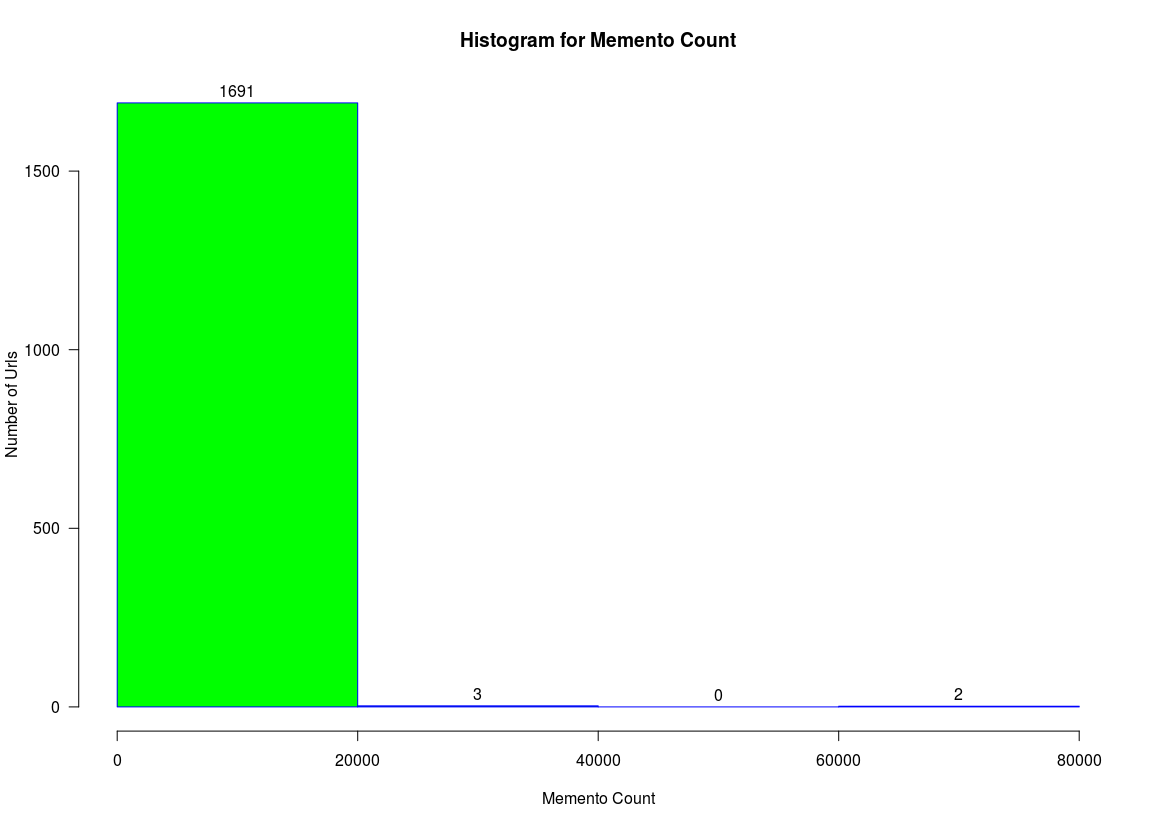
\includegraphics[width=0.9\textwidth, keepaspectratio]{MementoHistogram.png}
  \caption{Histogram for Memento Distribution}
  \label{Graph}
\end{figure}
   %}

\end{homeworkProblem}

%----------------------------------------------------------------------------------------
%   PROBLEM 3
%----------------------------------------------------------------------------------------

\begin{homeworkProblem}

Estimate the age of each of the 1000 URIs using the "Carbon
Date" tool:

\url{http://ws-dl.blogspot.com/2017/09/2017-09-19-carbon-dating-web-version-40.html}

Note: you should use "docker" and install it locally.  You can do
it like this:

\url{http://cd.cs.odu.edu/cd?url=http://www.cs.odu.edu/}

But it will inevitably crash when everyone tries to use it at the
last minute.

For URIs that have > 0 Mementos and an estimated creation date,
create a graph with age (in days) on the x-axis and number of
mementos on the y-axis.

Not all URIs will have Mementos, and not all URIs will have an
estimated creation date.  Show how many fall into either categories.
For example,

total URIs:         1000

no mementos:        137  

no date estimate:   212

%\problemAnswer
%{
    \begin{verbatim}\end{verbatim}
    \textbf{SOLUTION}\\

\begin{lstlisting}[language=Python, breaklines=true]
'''
Function to carbondate urls 
'''


def carbondate_urls():

    file_urls_expand = open("Urls_Uniq_Expanded.txt", "r")
    file_carbondate = open("Urls_carbondate.txt", "w")
    current_date = datetime.datetime.now()
    for line in file_urls_expand:
        try:
            command = "http://localhost:8888/cd/"
            command = command + line.rstrip().split("|||")[0]
            print(command)
            response = requests.get(command)
            if response.status_code == 200:
                print(response.text)
                carbon_date_result = ast.literal_eval(response.text)
                creation_date = carbon_date_result["estimated-creation-date"]
                creation_date = datetime.datetime.strptime(creation_date, "%Y-%m-%dT%H:%M:%S")
                print(creation_date)
                print(current_date)
                print((current_date - creation_date).days)
                file_carbondate.write(line.rstrip().split("|||")[0] + "|||" + str((current_date - creation_date).days) + "\n")
        except Exception as e:
            continue
    file_carbondate.close()
    file_urls_expand.close()
\end{lstlisting}

\begin{figure}[ht]
  \centering
  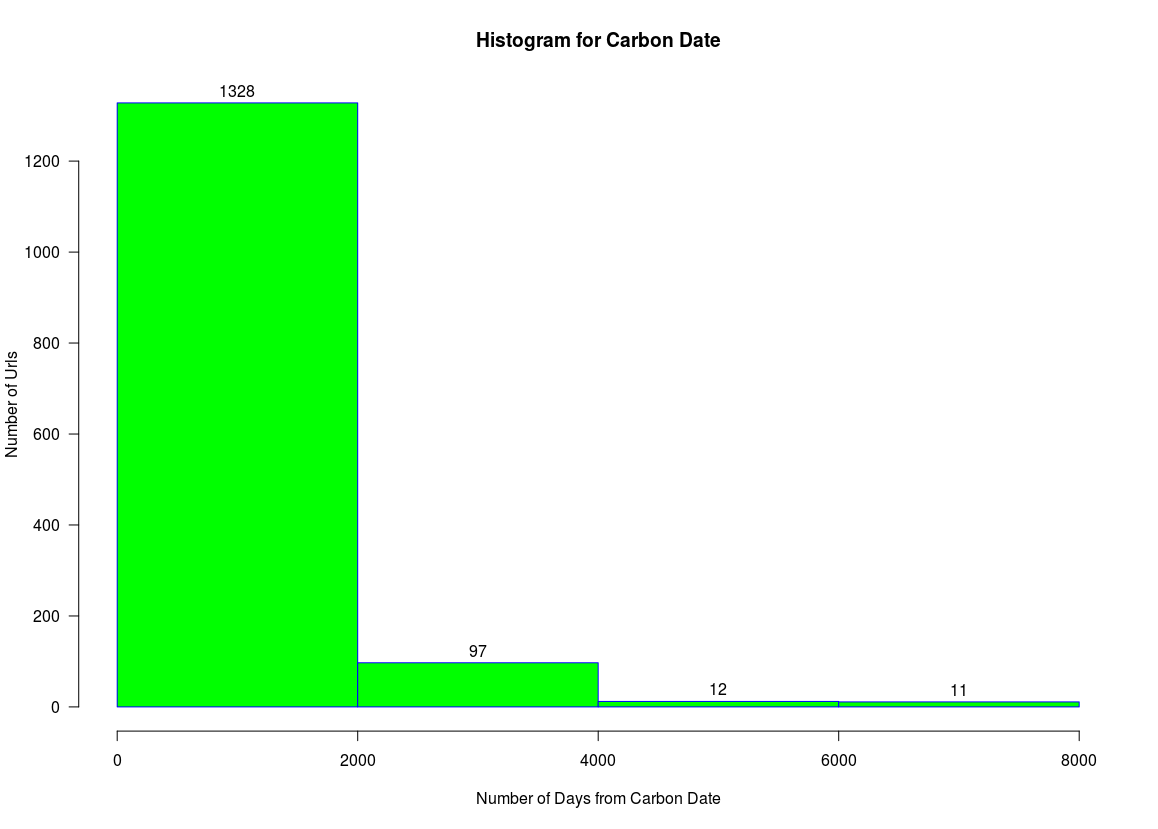
\includegraphics[width=0.9\textwidth, keepaspectratio]{Carbondate.png}
  \caption{Histogram for Carbon Date Distribution}
  \label{Graph}
\end{figure}
\begin{enumerate}
\item \textbf{Carbon Date}: All the urls were supplied to CarbonDate to find the earliest creation date from web archives. The earliest creation date returned was substracted with current date to know the number of days since the creation of the url. I could find creation dates for 1448 urls from 2088 urls.
\item \textbf{Histogram}: 1328 urls had a carbon date between 0 to 2000 days. 97 urls had a carbon date of 2000 to 4000 days. 12 urls had a carbon date of 4000 to 6000 days. 11 urls had a carbon date og 6000- 8000 days.
\end{enumerate}

\begin{center}
\begin{tabular}{ |c|c|c| } 
 \hline
 Total URI & 2088 \\ 
 No Mementos & 392 \\ 
 No date estimate & 640 \\ 
 \hline
\end{tabular}
\end{center}
\end{homeworkProblem}
\bibliographystyle{plain}
\bibliography{A2bibFile}

\end{document}
    


   

    

    

    
   
